\documentclass[12pt]{article}

\usepackage{array}
\usepackage{diagbox}
\usepackage{graphicx}
\usepackage{paralist}
\usepackage{amsfonts}
\usepackage{amsmath}
\usepackage{hhline}
\usepackage{booktabs}
\usepackage{multirow}
\usepackage{multicol}
\usepackage{color}

\newcommand{\ind}{\hspace*{0.6cm}}
\newcommand{\set}[1]{{\{\, #1 \,\}}}
\newcommand{\Implies}{\Rightarrow}
\newcommand{\rem}[1]{\textcolor{blue}{[#1 --- EH]}}

\oddsidemargin 0mm
\evensidemargin 0mm
\textwidth 160mm
\textheight 200mm
\renewcommand\baselinestretch{1.0}

\pagestyle {plain}
\pagenumbering{arabic}

\newcounter{stepnum}

\title{CS 2ME3 Assignment 4, Specification}
\author{Emily Horsman}

\begin {document}

\maketitle

This document contains a Module Interface Specification for the Model component
of the game `FreeCell'.
It assumes that a hypothetical View and Controller component exists but
contains no specification for these components.
Due to this assumption, there are some access programs in the modules below
which are not strictly necessary for the Model MIS, but would be necessary to
implement a View and Controller, and happen to be useful for unit testing.
These access programs are commented below.
\\\\
Instead of having a unique data structure (e.g., a Maybe/Optional type) for the
free cells, all placements in the game are represented with the same data
structure.
This is accomplished by having a bounded capacity on this data structure, which
is effective because no placement has an infinite bound anyway.
Checking this bound is useless on the foundation and cascade placements because
the rules for their valid moves would prevent the capacity from ever being
exceeded.
However, I feel that this bound increases the self-documentation of the
instances and is useful for having placements represented homogeneously.
\\\\
Different sources of the rules use different terminology for each placement in
the game. Below is the nomenclature of this document (diagram made with
draw.io).
\begin{center}
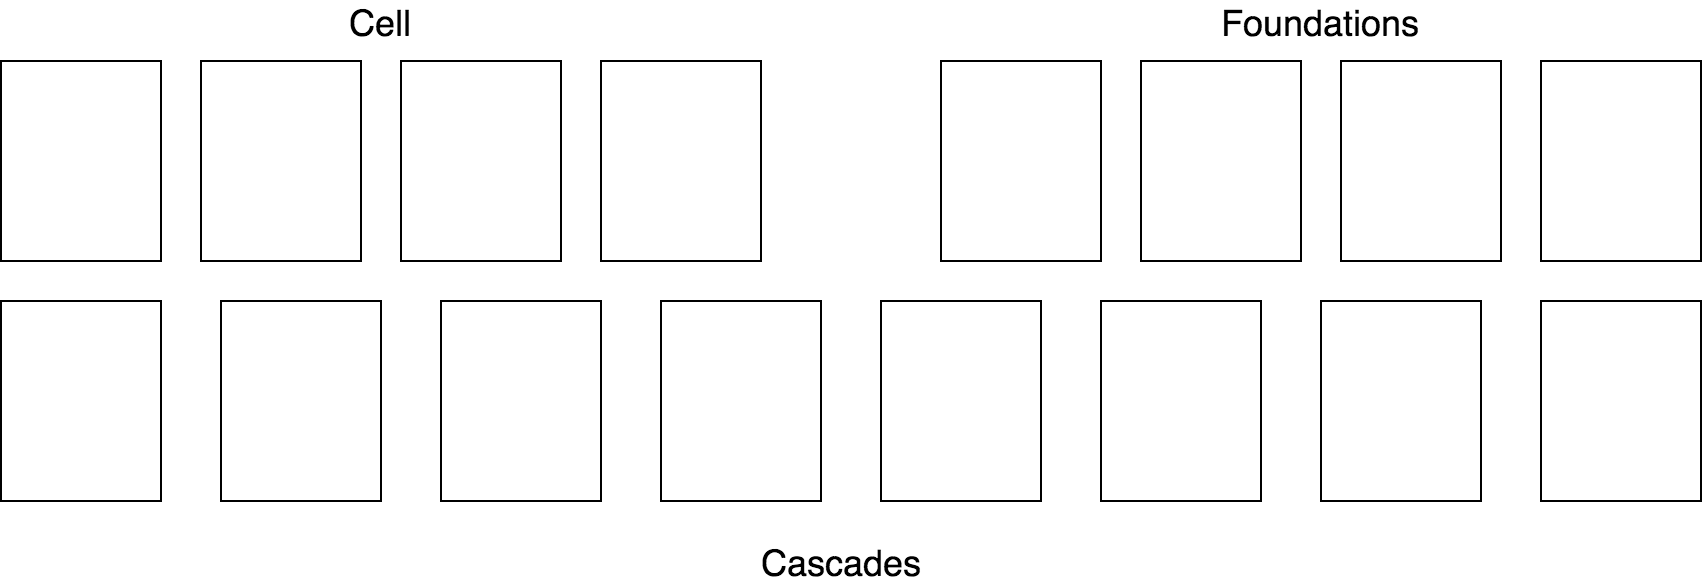
\includegraphics[width=0.9\textwidth]{NomenclatureDiagram.png}
\end{center}

\newpage

\section*{Game Types Module}

\subsection*{Module}

GameTypes

\subsection*{Syntax}

\subsubsection*{Exported Constants}

Ace : RankT = 1\\
Jack : RankT = 11\\
Queen : RankT = 12\\
King : RankT = 13\\

\subsubsection*{Exported Types}

PlacementT = \{ Cell, Foundation, Cascade \}\\
SuitT = \{ Spades, Clubs, Hearts, Diamonds \}\\
RankT = $\set{ n : \mathbb{N} \,|\, n \in [1, 13] : n }$\\

\subsection*{Semantics}

\subsubsection*{State Variables}

None

\subsubsection*{State Invariant}

None


\newpage


\section*{Generic Stack Module}

\subsection*{Generic Template Module}

StackADT(T)

\subsection*{Uses}

N/A

\subsection*{Syntax}

\subsubsection*{Exported Constants}

None

\subsubsection*{Exported Types}

Stack(T) = ?

\subsubsection*{Exported Access Programs}

\begin{tabular}{| l | l | l | l |}
\hline
\textbf{Routine name} & \textbf{In} & \textbf{Out} & \textbf{Exceptions}\\
\hline
Stack & $\mathbb{N}$ & Stack & invalid\_capacity\\
\hline
isEmpty & ~ & $\mathbb{B}$ & ~\\
\hline
isFull & ~ & $\mathbb{B}$ & ~\\
\hline
capacity & ~ & $\mathbb{N}$ & ~\\
\hline
push & T & ~ & full\\
\hline
peek & ~ & T & empty\\
\hline
pop & ~ & T & empty\\
\hline
seq & ~ & seq(T) & ~\\
\hline
\end{tabular}

\noindent\rem{seq() would be required for a hypothetical view.
isEmpty() and isFull() violate essentiality given that capacity() and seq()
exist, however I believe this violation gives a more understandable design which
is an acceptable tradeoff.}

\subsection*{Semantics}

\subsubsection*{State Variables}

s: seq of T\\
capacity: $\mathbb{N}$

\subsubsection*{State Invariant}

None

\subsubsection*{Assumptions}

\begin{itemize}
    \item The Stack(T) constructor is called for each object instance before
        any other access routine is called for that object.
\end{itemize}

\subsubsection*{Access Routine Semantics}

\noindent Stack($c$):
\begin{itemize}
    \item transition: $s, \mbox{capacity} := \left<\right>, c$
    \item output: $out := \mathit{self}$
    \item exception: $exc := (c = 0 \Implies \mbox{invalid\_capacity})$
\end{itemize}

\noindent isEmpty():
\begin{itemize}
    \item output: $out := |s| = 0$
    \item exception: None
\end{itemize}

\noindent isFull():
\begin{itemize}
    \item output: $out := |s| = \mbox{capacity}$
    \item exception: None
\end{itemize}

\noindent capacity():
\begin{itemize}
    \item output: $out := \mbox{capacity}$
    \item exception: None
\end{itemize}

\noindent push($v$):
\begin{itemize}
    \item transition: $s := s \,|| \left< v \right>$
    \item exception: $exc := (|s| = \mbox{capacity} \Implies \mbox{full})$
\end{itemize}

\noindent peek():
\begin{itemize}
    \item output: $out := s[|s| - 1]$
    \item exception: $exc := (|s| = 0 \Implies \mbox{empty})$
\end{itemize}

\noindent pop():
\begin{itemize}
    \item transition: $s := s[0..|s| - 2]$
    \item exception: $exc := (|s| = 0 \Implies \mbox{empty})$
\end{itemize}

\noindent seq():
\begin{itemize}
    \item output: $out := s$
    \item exception: None
\end{itemize}

\newpage


\section*{Card Module}

\subsection*{Template Module}

CardADT

\subsection*{Uses}

GameTypes for SuitT, RankT

\subsection*{Syntax}

\subsubsection*{Exported Constants}

None

\subsubsection*{Exported Types}

CardT = ?

\subsubsection*{Exported Access Programs}

\begin{tabular}{| l | l | l | l |}
\hline
\textbf{Routine name} & \textbf{In} & \textbf{Out} & \textbf{Exceptions}\\
\hline
CardT & SuitT, RankT & CardT & \\
\hline
suit & ~ & SuitT & ~\\
\hline
rank & ~ & RankT & ~\\
\hline
isRed & ~ & $\mathbb{B}$ & ~\\
\hline
\end{tabular}

\subsection*{Semantics}

\subsubsection*{State Variables}

s: SuitT\\
r: RankT

\subsubsection*{State Invariant}

None

\subsubsection*{Assumptions}

\begin{itemize}
    \item The CardT constructor is called for each object instance before
        any other access routine is called for that object.
\end{itemize}

\subsubsection*{Access Routine Semantics}

CardT($S, R$):
\begin{itemize}
    \item transition: $s, r := S, R$
    \item output: $out := \mathit{self}$
    \item exception: None
\end{itemize}

\noindent suit():
\begin{itemize}
    \item output: $out := s$
    \item exception: None
\end{itemize}

\noindent rank():
\begin{itemize}
    \item output: $out := r$
    \item exception: None
\end{itemize}

\noindent isRed():
\begin{itemize}
    \item output: $out := s \in \set{\mbox{Diamonds}, \mbox{Hearts}}$
    \item exception: None
\end{itemize}


\newpage


\section*{Game Module}

\subsection*{Template Module}

GameADT

\subsection*{Uses}

CardADT for CardT, StackADT for Stack,
GameTypes for PlacementT, Ace, King

\subsection*{Syntax}

\subsubsection*{Exported Constants}

None

\subsubsection*{Exported Types}

GameT = ?

\subsubsection*{Exported Access Programs}

\begin{tabular}{|l|>{\raggedright\arraybackslash}p{3.9cm}|l|p{3.5cm}|}
\hline
\textbf{Routine name} & \textbf{In} & \textbf{Out} & \textbf{Exceptions}\\
\hline
GameT & ~ & GameT & ~\\
\hline
GameT & seq(Stack(CardT)) & GameT & ~\\
\hline
hasWon & ~ & $\mathbb{B}$ & ~\\
\hline
isValidMove & PlacementT, $\mathbb{N}$, PlacementT, $\mathbb{N}$
            & $\mathbb{B}$ & invalid\_placement, empty\_source\\
\hline
noValidMoves & ~ & $\mathbb{B}$ & ~\\
\hline
performMove & PlacementT, $\mathbb{N}$, PlacementT, $\mathbb{N}$
            & ~ & invalid\_placement, invalid\_move\\
\hline
getCol & PlacementT, $\mathbb{N}$ & Stack(CardT) & invalid\_placement\\
\hline
\end{tabular}

\subsection*{Semantics}

\subsubsection*{State Variables}

cols: seq of Stack(CardT)

\subsubsection*{State Invariant}

None

\subsubsection*{Assumptions}

\begin{itemize}
    \item The GameT() constructor is called for each object instance before
        any other access routine is called for that object.
    \item Any seq(Stack(CardT)) value passed to the GameT(c) constructor will
        have been constructed from a previous GameT instance and is thus a valid
        board.
    \item Programs using this model specification are aware of the number of
        cascades, cells, and foundations. invalid\_placement will be thrown for
        an invalid configuration but there is no method to check whether a
        placement is valid or not because this is considered an axiom of the
        game and moves can only occur from interactions with the
        Controller/View.
\end{itemize}

\subsubsection*{Access Routine Semantics}

GameT():
\begin{itemize}
    \item transition: $
        \mbox{cols} := \mbox{rng(possibleCascades)} \,||\, \mbox{cells} \,||\, \mbox{foundations}$\\
        \ind where $\mbox{cells}, \mbox{foundations} :=
        \\\ind\ind ||( i : \mathbb{N} \,|\, i \in [0..3] : \left< \mbox{Stack}(1) \right> ),
        ||( i : \mathbb{N} \,|\, i \in [0..3] : \left< \mbox{Stack}(13) \right> )
        $
        \rem{Since the order of the sequence of same-Stack instances does not
        matter, $||$ can be used as the binary operator of a reduce/fold.}
    \item output: $out := self$
    \item exception: None
\end{itemize}

\noindent GameT($c$):
\begin{itemize}
    \item transition: $\mbox{cols} := c$
    \item output: $out := self$
    \item exception: None
\end{itemize}

\noindent hasWon():
\begin{itemize}
    \item output: $out := \forall\,( i : \mathbb{N} \,|\, i \in [12..15] :
        \\\ind \lnot \mbox{cols}[i].\mbox{isEmpty}() \land \mbox{cols}[i].\mbox{peek}().\mbox{rank}() = \mbox{King})$
    \item exception: None
\end{itemize}

\noindent isValidMove($p, i, q, j$):
\begin{itemize}
    \item output:

        \begin{tabular}[t]{|l|l|l|}
            \hhline{~|~|-|}
            \multicolumn{1}{r}{} & \multicolumn{1}{r|}{} & $out :=$\\
            \hhline{|-|-|-|}
            \multicolumn{1}{|l}{$q = \mbox{Cell}$} & ~ & dst.\mbox{isEmpty}()\\
            \hhline{|-|-|-|}
            $q = \mbox{Foundation}$ & $p = \mbox{Foundation}$ & false\\
            \hhline{|~|-|-|}
            ~ & $p \neq \mbox{Foundation}$ & $\mbox{isValidBuild}(src.\mbox{peek}(), j)$\\
            \hhline{|-|-|-|}
            \multicolumn{1}{|l}{$q = \mbox{Cascade}$} & ~ & $\mbox{isValidStack}(src.\mbox{peek}(), j)$\\
            \hhline{|-|-|-|}
        \end{tabular}

        where $src, dst := \mbox{getCol}(p, i), \mbox{getCol}(q, j)$
    \item exception: $exc := (\\\ind
        \lnot \mbox{isValidPlacement}(p, i) \lor
        \lnot \mbox{isValidPlacement}(q, j) \Implies \mbox{invalid\_placement} \,|\,\\
        \ind\mbox{getCol}(p, i).\mbox{isEmpty}() \Implies \mbox{empty\_source}\\)$
\end{itemize}

\noindent noValidMoves():
\begin{itemize}
    \item output: $out := \lnot \,\exists( p, q : \mbox{PlacementT}, i, j : \mathbb{N} \,|\,\\\ind
        \mbox{isValidPlacement}(p, i) \land \mbox{isValidPlacement}(q, j) :
        \mbox{isValidMove}(p, i, q, j))$
    \item exception: None
\end{itemize}

\noindent performMove($p, i, q, j$):
\begin{itemize}
    \item transition: $dst.\mbox{push}(src.\mbox{peek}()), src.\mbox{pop}()$\\\ind
        where $src, dst := \mbox{getCol}(p, i), \mbox{getCol}(q, j)$
        \rem{This is an operational specification to keep the spec readable
        and to avoid violating an interface.}
    \item exception: $exc := (\\\ind
        \lnot \mbox{isValidPlacement}(p, i) \lor
        \lnot \mbox{isValidPlacement}(q, j) \Implies \mbox{invalid\_placement} \,|\,\\\ind
        \lnot \mbox{isValidMove}(p, i, q, j) \Implies \mbox{invalid\_move}\\)$
\end{itemize}

\noindent getCol($p, i$):
\begin{itemize}
    \item output:
        \begin{tabular}[t]{|l|l|}
            \hhline{~|-|}
            \multicolumn{1}{r|}{} & $out :=$\\
            \hhline{-|-|}
            $p = \mbox{Cascade}$ & $\mbox{cols}[i]$\\
            \hhline{|-|-|}
            $p = \mbox{Cell}$ & $\mbox{cols}[i + 8]$\\
            \hhline{|-|-|}
            $p = \mbox{Foundation}$ & $\mbox{cols}[i + 12]$\\
            \hhline{|-|-|}
        \end{tabular}
    \item exception: $exc := (\lnot \mbox{isValidPlacement}(p, i) \Implies \mbox{invalid\_placement})$
\end{itemize}

\subsection*{Local Functions}

isValidPlacement: $\mbox{PlacementT} \rightarrow \mathbb{N} \rightarrow \mathbb{B}$\\
\noindent isValidPlacement($p, i$) $\equiv$\\
\ind$(p = \mbox{Cell} \lor p = \mbox{Foundation} \Implies 0 \leq i \leq 3 \,|\, p = \mbox{Cascade} \Implies 0 \leq i \leq 7)$
\\\\
isValidBuild: $\mbox{CardT} \to \mathbb{N} \to \mathbb{B}$\\
\noindent isValidBuild($c, j$) $\equiv (\\
\ind s.\mbox{isEmpty}() \Implies c.\mbox{rank}() = \mbox{Ace} \,|\,\\
\ind\lnot s.\mbox{isEmpty}() \Implies
(s.\mbox{peek}().\mbox{suit}() = c.\mbox{suit}() \land
s.\mbox{peek}().\mbox{rank}() = c.\mbox{rank}() - 1)\\)$\\
where $s := \mbox{getCol}(\mbox{Foundation}, j)$
\\\\
isValidStack: $\mbox{CardT} \to \mathbb{N} \to \mathbb{B}$\\
\noindent isValidStack($c, j$) $\equiv (\\\ind
s.\mbox{isEmpty}() \mid\\\ind
\lnot s.\mbox{isEmpty}() \Implies (s.\mbox{peek}().\mbox{isRed}() \neq c.\mbox{isRed}() \land
s.\mbox{peek}().\mbox{rank}() - 1 = c.\mbox{rank}())\\)$\\
where $s := \mbox{getCol}(\mbox{Cascade}, j)$
\\\\
isDistinct: $\mbox{Stack(CardT)} \to \mbox{Stack(CardT)} \to \mathbb{B}$\\
\noindent isDistinct($a, b$) $\equiv
\lnot \exists(i, j : \mathbb{N}, c, c' : \mbox{CardT} \,|\,\\\ind
    i \in [0..|a.\mbox{seq}()| - 1] \land j \in [0..|b.\mbox{seq}()| - 1] \land
    c = a.\mbox{seq}()[i] \land c' = b.\mbox{seq}()[j]\\\ind
    : c.\mbox{suit}() = c'.\mbox{suit}() \land c.\mbox{rank}() = c'.\mbox{rank}()
\\)$
\\\\
possibleCascades: $\mbox{seq(Stack(CardT))}$\\
possibleCascades $\equiv \{ s : \mbox{seq(Stack(CardT))} \,|\,$\\
\ind$|s| = 8 \land \\
\ind\forall( i : \mathbb{N} \,|\, i \in [0..7] : s[i].\mbox{capacity}() = 19) \land\\
\ind\forall( i : \mathbb{N} \,|\, i \in [0..3] : |s[i].\mbox{seq}()| = 7) \land\\
\ind\forall( i : \mathbb{N} \,|\, i \in [4..7] : |s[i].\mbox{seq}()| = 6 )\, \land\\
\ind\forall( i, j : \mathbb{N} \,|\, i, j \in [0..7] \land i \neq j : \mbox{isDistinct}(s[i], s[j]))\\
: s \}$
\rem{This produces a set of all possible board configurations so that one can
be chosen at randomly. The range expression of this set comprehension denotes
what a valid initial sequence of cascade stacks looks like.}
\\\\
rng: $\mbox{set(T)} \to \mbox{T}$\\
\noindent rng($s$) $\equiv$ a random member of the set $s$ with each member
having a $1/|s|$ probability of being chosen


\end{document}
